\chapter{Modelling}
\label{chap:model}

This chapter describes the representations of our models. Requirement Engineering goal models are generally discussed in meeting rooms on white boards, coffee shops on back of napkins or over phone conferences. Since they are mostly crude and rudimentary, we developed a python based framework to support representing these models for our experiments. These representations are concise for business users to encode in and elaborate enough for engineers to work with. The notations are available online in our repository\footnote{\url{https://github.com/ai-se/softgoals}}.

\section{i*}
\label{sec:model:i*}

i* modelling framework was described briefly in section \ref{subsec:bg:gm:istar}.\fref{fig:istar} shows a sample i* model Model for youth counselling. The model was originally from Horkoff Et. al's \cite{horkoff12} on Interactive Goal Model Analysis. The legend in the top right corner of the figure highlights various components of the model. The model essentially is a graph with nodes the decisions to be taken and the stakeholders' requirements and the edges representing the relationship between them.

\begin{table}[htpb]
\centering
\begin{tabular}{|c|c|c|c|}
\hline
\textbf{Nodes}    & \textbf{Values}                                                                                         & \textbf{Incoming Edges}                                             & \textbf{Outgoing Edges}                                                             \\ \hline
\textbf{Task}     & \begin{tabular}[c]{@{}c@{}}Satisfied\\ Unsatisfied\end{tabular}                                                    & \begin{tabular}[c]{@{}c@{}}Dependency\\ Decompositions\end{tabular} & \begin{tabular}[c]{@{}c@{}}Dependency\\ Decompositions\\ Contributions\end{tabular} \\ \hline
\textbf{Resource} & \begin{tabular}[c]{@{}c@{}}Satisfied\\ Unsatisfied\end{tabular}                                                    & \begin{tabular}[c]{@{}c@{}}Dependency\\ Decompositions\end{tabular} & \begin{tabular}[c]{@{}c@{}}Dependency\\ Decompositions\\ Contributions\end{tabular} \\ \hline
\textbf{Goal}     & \begin{tabular}[c]{@{}c@{}}Satisfied\\ Unsatisfied\end{tabular}                                                    & \begin{tabular}[c]{@{}c@{}}Dependency\\ Decompositions\end{tabular} & \begin{tabular}[c]{@{}c@{}}Dependency\\ Decompositions\\ Contributions\end{tabular} \\ \hline
\textbf{Softgoal} & \begin{tabular}[c]{@{}c@{}}(Partially) Satisfied\\ (Partially) Denied\\ Conflict\\ Unknown\end{tabular} & \begin{tabular}[c]{@{}c@{}}Dependency\\ Contributions\end{tabular}  & \begin{tabular}[c]{@{}c@{}}Dependency\\ Contributions\end{tabular}                  \\ \hline
\end{tabular}
\caption{Nodes and their representations in py*.}
\label{tab:pystar:nodes}
\end{table}

The nodes in the i* modelling framework are described in \tref{tab:pystar:nodes}. There are 4 kinds of nodes in the framework; \bit{Tasks}, \bit{Resources}, \bit{Goals} and \bit{Softgoals}. Tasks and Resources are treated as inputs to the model(decisions) provided they do not depend on any other task or resource in the graph. Goals and Softgoals characterize the stakeholders requirements(objectives). Goals are definitive in nature and its satisfiability can be quantified. Softgoals on the other hand are subjective in nature and their satisfiability can only be estimated. The satisfiability of node is determined or estimated by propagating the values of its corresponding source nodes through the edges.

\begin{table}[htpb]
\centering
\begin{tabular}{|c|c|c|}
\hline
\textbf{Edges}      & \textbf{Category} & \textbf{Comment}                                    \\ \hline
\textbf{Dependency} & Dependency        & Source node has to be satisfied.                    \\ \hline
\textbf{AND}        & Decomposition     & All the source nodes have to be satisfied.          \\ \hline
\textbf{OR}         & Decomposition     & Atleast one of the source node has to be satisfied. \\ \hline
\textbf{Make}       & Contribution      & Source node heavily supports destination.           \\ \hline
\textbf{Help}       & Contribution      & Source node weakly supports destination.            \\ \hline
\textbf{Hurt}       & Contribution      & Source node weakly hinders destination.             \\ \hline
\textbf{Break}      & Contribution      & Source node heavily hinders destination.            \\ \hline
\end{tabular}
\caption{Edges and their description in py*.}
\label{tab:pystar:edges}
\end{table}


\begin{table}[htpb]
\centering
\begin{tabular}{|c|c|c|c|c|c|}
\hline
\multicolumn{2}{|c|}{\textbf{Source Label}} & \multicolumn{4}{c|}{\textbf{Contribution Link Type}}           \\ \hline
\textbf{}        & \textbf{Name}            & \textbf{Make} & \textbf{Help} & \textbf{Hurt} & \textbf{Break} \\ \hline
\textbf{S}       & Satisfied                & \textbf{S}    & \textbf{PS}   & \textbf{PD}   & \textbf{PD}    \\ \hline
\textbf{PS}      & Partially Satisfied      & \textbf{PS}   & \textbf{PS}   & \textbf{PD}   & \textbf{PD}    \\ \hline
\textbf{C}       & Conflict                 & \textbf{C}    & \textbf{C}    & \textbf{C}    & \textbf{C}     \\ \hline
\textbf{U}       & Unknown                  & \textbf{U}    & \textbf{U}    & \textbf{U}    & \textbf{U}     \\ \hline
\textbf{PD}      & Partially Denied         & \textbf{PD}   & \textbf{PD}   & \textbf{PS}   & \textbf{PS}    \\ \hline
\textbf{D}       & Denied                   & \textbf{D}    & \textbf{PD}   & \textbf{PS}   & \textbf{PS}    \\ \hline
\end{tabular}
\caption{Propagation Rules for Contribution in py*}
\label{tab:pystar:props}
\end{table}

Edges in the graph are described in \t1ref{tab:pystar:edges}. There are essentially three kinds of edges; \bit{Dependencies}, \bit{Decompositions} and \bit{Contributions}. For a dependency edge, the target node will be satisfied if and only if the source node is satisfied. Decompositions are of two types; \bit{AND} and \bit{OR}. For an AND decomposition, all of the source nodes needs to be satisfied and incase of an OR decomposition, atleast one of the source node needs to be satisfied. Contribution links are subjective in nature, i.e a contribution link does not exactly justify the relation between the source and the destination rather gives an estimate on the relation. Contribution links are of four types; \bit{make}, \bit{help}, \bit{hurt} and \bit{break}. Make link shows that the source greatly supports the destination; help link shows that the source weakly supports the destination; hurt link shows that the source weakly hinders the destination; and break link shows that the source heavily hinders the destination.

Satisfiability based on contribution links is again subjective in nature. Giorgini Et. al highlighted the extent of satisfiability of a softgoal based on the incoming contribution links \cite{sebastiani2004}. This is described in \tref{tab:pystar:props}. If a node as multiple incoming contribution links resulting in conflicting contributions the node is said to have a ``conflict".

These definitions were used to build a modelling framework called \textbf{py*} and is publicly available for the community's experiments and analysis\footnote{\url{https://github.com/ai-se/softgoals/tree/master/src/pystar}}.

\section{Analytic Hierarchy Process}
\label{sec:model:ahp}

AHPs are another modelling framework we have explored in this thesis for optimizing design decisions. The semantics for AHP was illustrated in section \ref{subsec:bg:gm:ahp} and for the models we consider in our experiments we deal with multiple criteria(or objectives) for each models. In the example model, a software system has to be modernized and there are two approaches that the analysts can take; (1) Perform an incremental rewrite or (2) Big Bang rewrite. The requirements could be coarsely defined as maximizing benefit and minimizing cost in modernizing.

\begin{figure}[hbtp]
    \centering
    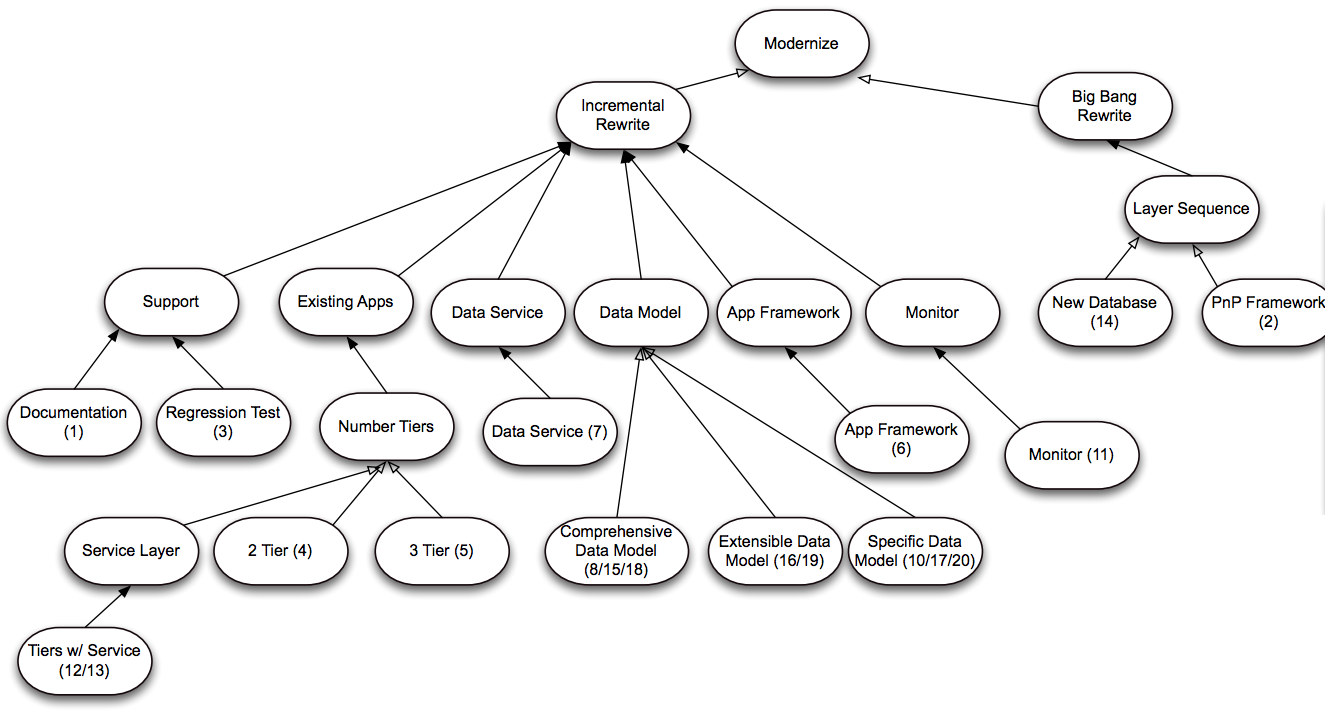
\includegraphics[width=\textwidth]{Chapter-3/figs/AHP}
    \caption{Sample AHP Model}
    \medskip
    \small
    The model highlights the options user has to 
    \label{fig:ahp}
\end{figure}

AHPs are represented as a tree with the prime decision in the root and all other sub-decisions leading up to it either through AND or OR edges. The AND and OR edge is similar to the i* model, requiring all and atleast one child node to be satisfied respectively. The cost and benefit presented by including a satisfied child node is cummulative and propagated to the root node. The leaf nodes are the decisions in the model that are set by the analysts.

AHPs are way simpler compared to i* models since they are both more concise and reduces ambiguity. This concise nature of the model causes the business analyst to define the model in an extremely accurate manner and asks forces them to resolve subjective conflicts while constructing the model.

The semantics based on the definition of an AHP model is encoded into a python based framework for analysis and future experimentation and is available publicly.\footnote{\url{https://github.com/ai-se/softgoals/tree/master/src/pyAHP}}